\chapter{A framework for analyzing the reproducibility issues of neuroimaging pipelines}
The Repro-tools \todo{name subject to change } is a framework developed for analyzing the reproducibility issues occurring in the neuroimaging pipelines. Though this framework is developed with various neuroimaging pipelines in focus, in principle, it can be also be used for analyzing data belonging to various other disciplines. The term `condition` with respect to this framework refers to different operating systems on which the data processing takes place. Likewise, the term `subject' with respect to this framework is used to denote the directories that are kept under each condition. 

My contribution to this framework is a script, called verifyFiles\footnote{\url{https://github.com/big-data-lab-team/repro-tools/blob/master/verifyFiles.py}}, which could compare the subjects processed under different conditions. The result of this comparison can give a summary of files that has differences due to the operating system on which the processing took place.

The script works under the assumption that, under an ideal scenario, files belonging to each subject is supposed to have equal checksum under different conditions. Repro-tools help in identifying the files having differences by comparing the checksum values of files stored under different conditions. This tool can also check for corruption of files. It can compute the checksum locally and compare it against the recorded checksum to find if the files are corrupted or not.

It can also quantify the differences in image files with the help of metrics like sum of squared distances (SSD), Dice coefficient etc. Additional metrics can be configured which could be used for quantifying differences occurring in different types of files. Repro-tools can also trace the provenance of these files having the differences. It helps us identify the processes that wrote the files having differences. Provenance tracing is done with the use of data captured by Reprozip.

%Refer what is subject also in the above paragraph
%Compute Canada in architecture

\begin{center}
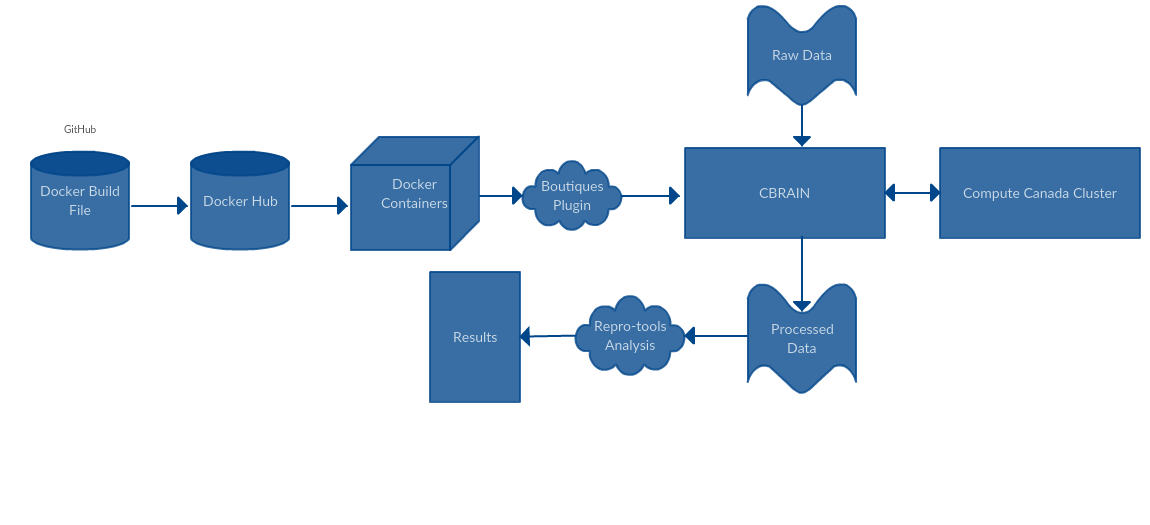
\includegraphics[width=\linewidth]{framework_architecture.png}
\captionof{figure}{Framework Architecture}
\label{fig:framework_architecture}
\end{center}

Figure \ref{fig:framework_architecture} illustrates the overall workflow. The Docker image creation is automated. For each commit, made to the Dockerfile stored in Github\footnote{\url{https://github.com/big-data-lab-team/Dockerfiles-HCP-PreFreesurfer}}, a new build is triggered in Dockerhub\footnote{\url{https://hub.docker.com/r/bigdatalabteam/hcp-prefreesurfer/}}. These images are then used by CBRAIN for processing the subjects. Boutiques helps in deploying these containers to CBRAIN platform. CBRAIN can harness the power of computational clusters as well. The subjects processed under different conditions are then analyzed using the Repro-tools.

\subsection{Docker images}
Our framework uses Docker containers for reproducibility studies. A Docker container is the running instance of a Docker image. Dockerfiles are used for specifiying the operating system and the libraries needed for each docker image. Whenever a commit is made to the Dockerfile, a new build gets triggered in the Dockerhub. Thus, the automated build makes sure that the changes are always reflected in the Docker images. The most notable advantage of hosting the Docker images on Dockerhub is that the repositories that are public can be used by anyone. 

Repro-tools, before the beginning of processing a subject, makes a check to ensure that the image that is getting used is the latest one. This check makes sure that the processing is done with the up-to-date changes in the Docker images.

\section{Pipeline Encapsulation}
I created a wrapper script\footnote{\url{https://github.com/big-data-lab-team/Dockerfiles-HCP-PreFreesurfer/blob/master/PreFreeSurfer-DockerFiles/command-line-script.sh}} on top of the HCP Pipelines to have the features which are listed below,
\begin{itemize}
  \item Compute the checksum of the files in each subject before and after the execution
  \item Create execution directory and copy the subject to prevent corrupting the input data
  \item Record all the software (library versions) present in the container and hardware specifications of the workstation
  \item Ability to trace the execution using Reprozip (optional)
\end{itemize}

The checksums were computed before and after execution so that corruption check can be done with the use of recorded checksums. After the execution directory creation, the subject folder is copied into the execution directory and thus, it prevents the corruption of the HCP data. Another feature, recording of the software library versions and hardware specifications are done in order to make sure that the only factor that changes in these experiments is the operating system version. The optional Reprozip tracing feature is used to record the details of the HCP Processing so that it is used as referrence for provenance tracing.

\section{Pipeline Deployment}
The Docker container containing the HCP Pipeline along with the Boutiques descriptor was deployed on a server setup as part of our study. With the help of CBRAIN along with the containers and the descriptors, we were able to process HCP subjects. Single server was used in order to prevent differences occurring in the files due to differences arising from the hardware architecture. Boutiques descriptors used for deploying the HCP Pipelines on CBRAIN is available at \cite{HCP_descriptors}.

%\begin{itemize}
 % \item Single server to ensure no hardware differences
  %\item Able to process multiple subjects at once
  %\item CBRAIN HCP plugins available here
%\end{itemize}

\section{File comparisons across conditions}
%Checksum
Repro-tools framework can compare the files across different conditions based on the checksum. We have used MD5\footnote{\url{https://tools.ietf.org/html/rfc1321}} algorithm for calculating the checksum of files. The output of a MD5 algorithm is a 128-bit ``fingerprint" or ``message digest"~\cite{md5}.


HCP subjects processed under different conditions are kept in different directories. The basic check is making sure that the files are common to all conditions for comparison. A pair of condition is taken at a time for comparison. The checksum of the files are recorded before and after the processing. Repro-tools can compute the checksums locally as well. 

Two types of differences can occur due to the minimal preprocessing. One is inter-OS difference which occur due the the operating system library updates and the other type, intra-OS differences occur due to pseudo-random processes used in the pipelines. Repro-tools can be used to identify both kind of differences.

The first step is identification of files with differences in their checksums. For the files that are identified to have differences, different kind of metrics are used base on the file type to quantify the differences. Normalized root mean square error, Dice Coefficient, Text filter etc. are the various metrics used for quantifying the differences. Section \ref{sec:num1} explains the metrics in detail. 

These metric values help us understand how big or small the differences are. Apart from quantifying the differences using type specific metrics, Repro-tools can also be used to trace the provenance of these differences. It is able to identify all the processes and associated parameters. These detailed information is helpful in debugging since we can recreate the processing step by step and identify the processes that creates the differences.

%\begin{itemize}
 %\item Identify the files that are common to all subjects and all conditions
 %\item Check intra-OS variability (e.g., due to pseudo-random processes)
 %\item Identifies files with differences (based on md5 checksum)
 %\item Associates file types with specific metrics (Normalized RMSE, Text filters, Dice coefficient)
 %\item Computes difference matrix for each metric and associates matrix with Reprozip trace
%\end{itemize}

\section{Provenance Capture}
According to~\cite{Ikeda:2010:PSP:1855795.1855800}, ``provenance captures where data came from, how it was derived, manipulated, and combined, and how it has been updated over time". Provenance information can be used to explain the source or evolution of a data set. Thus it can help in generating a deeper understanding of the data set. It can also be used to verify and confirm that there were no bugs in the processing. Provenance information can be used to identify the bugs in the processing. Thus it can help in recomputing the steps that got corrupted and send the corrected data downstream~\cite{Ikeda:2010:PSP:1855795.1855800}.

The data recorded by Reprozip is recorded in an SQLite\footnote{\url{https://www.sqlite.org/}} database. Repro-tools framework queries this database to find out the provenance information about the files that has a difference in their checksum. Figure \ref{fig:provenance-query} contains the query used for finding the provenance information.\\

\begin{tcolorbox}[colback=black!5!white,colframe=black!75!black]
SELECT DISTINCT executed\_files.name, executed\_files.argv, executed\_files.envp, executed\_files.timestamp, executed\_files.workingdir from executed\_files INNER JOIN opened\_files where opened\_files.process = executed\_files.process and opened\_files.name like ? and opened\_files.mode=2 and opened\_files.is\_directory=0',('\%/'+file\_name,)
\end{tcolorbox}
\captionof{figure}{Query for provenance information}
\label{fig:provenance-query}

Query makes use of details about the 1) processes that wrote the file; 2) command line arguments used by those processes; 3) Environment variables used; 4) timestamp; 5) working directory. By the help of the details we get out of the query, we can reproduce the steps to debug the processes that create these differences.

\section{Metrics} \label{sec:num1}
The metrics that are used to quantify the differences are described below.

\subsection{Normalized Root Mean Square Error (NRMSE)}
As defined in \cite{khosrow2017handbook}, ``The Root Mean Square Deviation (RMSD) or root-mean-square error (RMSE) is a frequently used measure of the difference between values predicted by a model or an estimator and the values actually observed". Normalizing the RMSD value makes it easier to compare between models or datasets.

Example from \cite{NRMSE}, the RMSE of predicted values ${\displaystyle {\hat {y}}_{t}}$  for times t of a regression's dependent variable ${\displaystyle y_{t}}$ is computed for n different predictions as the square root of the mean of the squares of the deviations:\\

\begin{center}
  \begin{equation}
     RMSE = {\sqrt {\frac{1} {n}{\sum\limits_{t = 1}^n {(\hat{y}_{t} - {y}_{t} } })^{2} } }
  \end{equation}
\end{center}

\begin{center}
  \begin{equation}
    NRMSE = {\frac{RMSE} {y_{max} - y_{min}}}
  \end{equation}
\end{center}

\subsection{Dice Similarity Coefficient}
Dice Similarity Coefficient can be used as a statistical validation metric for measuring the reproducibility of magnetic resonance images~\cite{Zou2004}.
\begin{center}
  \begin{equation}
     J(A,B) = {{|A \cap B|}\over{|A \cup B|}} = {{|A \cap B|}\over{|A| + |B| - |A \cap B|}}
  \end{equation}
\end{center}
\begin{itemize}
\item NRMSE
\item Dice
\end{itemize}
